\section{Thursday, 13 December 2018}

\subsection{Steps}
After trying different methods of classification and prediction we proceed to analyze them and see which obtain a best prediction.
\begin{itemize}
	\item \textbf{\textit{Naive Bayes}: } 
	\begin{figure}[H]
		\centering
		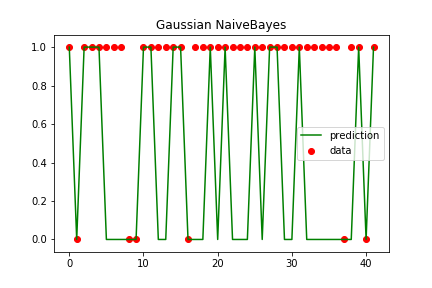
\includegraphics{../../reports/figures/NaiveBayesPrediction}
		\caption{Naive Bayes prediction}
	\end{figure}
	This is the algorithm which predicts more attacks. In addition, there are very few false positives. It has a error measure of 0.12 approximately, so it means that 12 values of 100 are incorrectly predicted.
	\item \textbf{\textit{KNN:}}
		\begin{figure}[H]
		\centering
		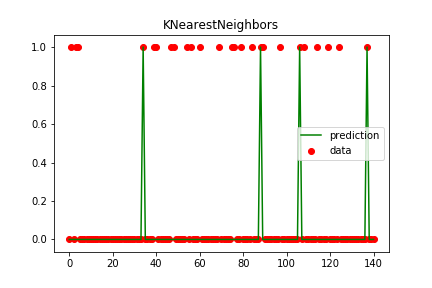
\includegraphics{../../reports/figures/KNearestNeighborsPrediction}
		\caption{KNearest Neighbors prediction}
	\end{figure}
	We obtain an insignificant error measure such as 0.07. It seems is a perfect algorithm because it always hits the prediction, but we can see in the graph that it only predicts when there are no attacks. In spite of that, when it predicts an attack it is usually correct.
	\item \textbf{\textit{Random Forest:}}
	\begin{figure}[H]
		\centering
		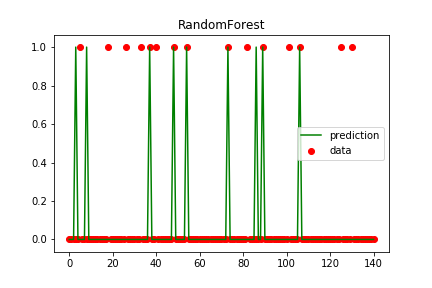
\includegraphics{../../reports/figures/RandomForestPrediction}
		\caption{Random Forest prediction}
	\end{figure}
	As in the algorithm \textit{KNN} it has a very low error. In this one, more false positives are observed and it not predict enough attacks.
\end{itemize}
The best algorithm to predict attacks is \textit{Naive Bayes} since it predicts more attacks and although it has a greater error than the other two it is still very low. With a better training model we could predict more attacks, but in this case the data with attacks are significantly lower than those that don't receive attacks.